% Image wrapper: PDF table structure was not recoverable automatically.
% Requires \usepackage{graphicx}. Replace the image with tabular cells when editable text is needed.
% Caption: TableX.Theproposedmodelachievesthebestresultson both the dehazing and denoising tasks. Compared to the recent MoCE-IR [29], which adopts a mixture-of-experts strategy for improvedefficiency,ourapproachachievesanaveragePSNR gainof0.18dBacrossalldegradationtypesandanotable improvementof0.85dBonthedehazingtask.Thissuperior performanceisachievedwithonly29\%oftheparameters, highlighting the efficiency of our design. 2)Five-TaskSetting:Wefurtherevaluateourmodelunder amorechallengingfive-tasksettingbyadditionallyincluding motion deblurring and low-light image enhancement. As shown inTableXI,ourmethodachievesthebestresultsonmost datasets.Whenaveragedacrossalldatasets,itsurpassesthe smallversionofMoCE-IR[29]by0.62dBinPSNR.Even compared with its normal version, our model achieves a 0.12 dB improvement while reducing parameters by 71\%. Furthermore, it outperforms the recent AdaIR [25], which leverages frequency priors to boost performance, on all metrics while using only 26\% of the parameters. The visual results on the real LOLv1 [97] dataset are shown in Fig. 7. Our model is able to recover richer structural and textural details from the challenging low-light images compared with the recent frequency-based AdaIR [25], producing clearer and more visually faithful restorations. 3)GeneralizationEvaluation:Toassessthegeneralization capabilityofourmodel,wefollow[25],[26]anddirectly applythemodelpre-trainedunderthefive-tasksettingtotwo additional denoising datasets: Urban100 [98] and Kodak24 [99]. Table XII shows that our model attains the highest scores on both datasets, outperforming strong competitors. In particular, under
\begin{tabular}{c}
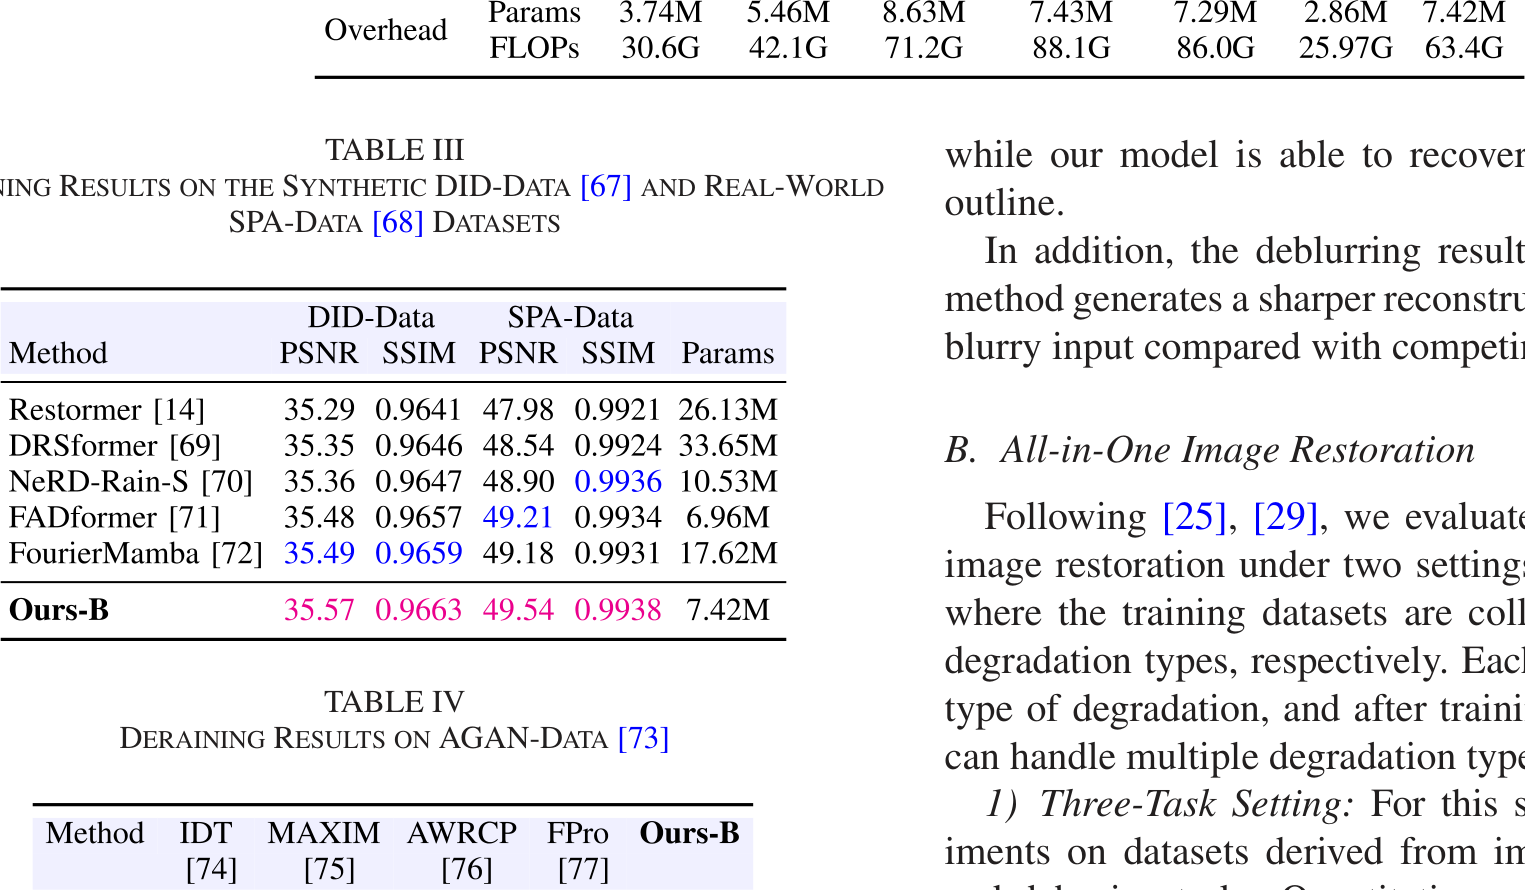
\includegraphics[width=\linewidth]{../original/Table10_p006.png}
\end{tabular}
